\documentclass{article}
\usepackage[14pt]{extsizes}
\usepackage[T2A]{fontenc}
\usepackage[utf8]{inputenc}
\usepackage[english, russian]{babel}
\usepackage[left=3cm,right=1.5cm,top=2cm,bottom=2cm]{geometry}
\usepackage{hyperref}
\usepackage{amsmath}
\usepackage{cleveref}
\usepackage{caption}


\usepackage{graphicx}

%\полуторный интервал
\usepackage{setspace}
\onehalfspacing

%простое дерево
\usepackage{dirtree}

%формулы
\usepackage{mathtools}
\usepackage{amsfonts}
% \everymath{\displaystyle}

%красные строки (не рекомендуется)
% \parindent = 1,25cm
% \usepackage{indentfirst}

\begin{document}
%\input{title}
\tableofcontents
\newpage

\section{System architecture}

\subsection{Обработка гомогенных и гетерогенных данных}
\begin{quote}
    Homogeneous Data Structures: This type can only store a single type of data inside them(integer, character, etc.), Heterogeneous Data Structures: This type can store more than one type of data at the same.
\end{quote}

Основным принципом работы классических баз данных является обращение к памяти на физическом устройстве.
с помощью индекса (например хеш функции). Основой таких баз данных является реляционная алгебра.\\
\textbf{Реляционные базы данных} используют таблицы для хранения строго структурированных данных.\\
\textbf{Структурированные данные} предполагают наличие определенной схемы (определяется при создании базы данных) и типа данных.\\

Но с развитием реляционных баз данных были введены новые полуструктурированные данные, которые могут содержать наборы данных с бесконечными(динамическими) значениями, состоять из других объектов данных. С дальнейшем
развитием технологий возникает понятие NoSQL, которые могут работать с слабоструктурированными и неструктурированными объектами. \textbf{Например: } фильм, аудиофайл.\\
Один из таких типов данных это поток данных записываемых в базу данных.\\
\textbf{Поток данных} - это поток данных с изменяемым числом записей в секунду(any unit of time). Особенностью таких данных является то что обрабатывать такие данные можно только последовательно.\\

На изображении \ref{img1} показана система аукциона представляемая потоком данных. Ставки имеют объем в валюте и временю метку. Затем будет выбран пользователь что сделал наибольшую ставку. А поток данных можно использовать для дальнейшего анализа.
\newpage

\begin{figure}[h]
    \centering
    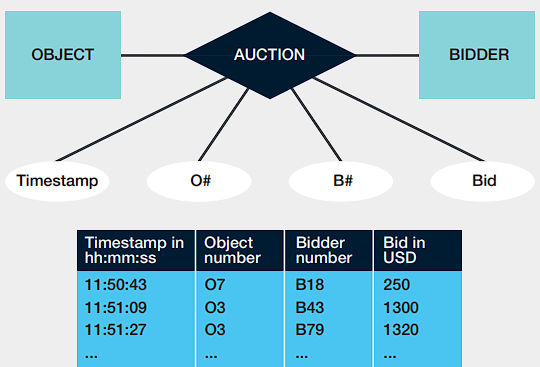
\includegraphics[width=0.7\textwidth]{images/datastream.png}
    \caption{Поток данных}
    \label{img1}
\end{figure}

\textbf{Неструктурированные данные} - данные без структуры, например снимки с спутников, музыкальные файлы. Чаще всего такие данные возникают в процессах big data. Хранилища данных для таких типов являются NoSQL.

\subsection{Структуры хранения и доступа}
\begin{quote}
    Storage and access structures for relational and nonrelational database systems should 
    be designed to manage data in secondary storage as efficiently as possible.
\end{quote}

\subsubsection{Структуры: индекс, дерево}
\textbf{Индекс атрибута} это структура, которая эффективно предоставляет для каждого значения атрибута, внутренний адрес для всех записей имеющих такое значение атрибута.\\
\textbf{Пример:} сортированная нумерация, отсортированные по алфавиту строки.\\

\textbf{Структуры вида дерево} позволяют хранить записи или индексы для увеличения эффективности. Для получения записи необходимо выполнить операцию поиска по дереву.
В классической реализации дерево состоит из корневого узла и внутренних узлов, каждый из которых имеет 2 поддерева(бинарное дерево).
Проблема таких деревьев в высокой скорости роста высоты, а следовательно и количества запросов для доступа к данным. Для решения этой проблемы деревья предложено расширять в ширину а не высоту.
Одной из структур реализующих этот подход является B-tree.\\
\textbf{B-tree} - дерево в котором каждый узел имеет более 2ух поддеревьев. Где внутренние узлы и листья дерева не пусты.
B-tree $n$ ого порядка назовем дерево если:
\begin{enumerate}
    \item оно полностью сбалансировано (путь от корня до каждого листа имеет одинаковую длину)
    \item каждый внутренний узел имеет хотя бы $n$ и максимум $2*n$ вхождений в его data page.
\end{enumerate}
На рисунке \ref{img2} показано:
\begin{enumerate}
    \item Как таблица обращается в дерево индексов. Для нашего дерева $n = 2$ значит мы храним максимум 4 элемента в узле.
    \item Затем производится попытка добавить элемент, но т.к размер дерева $n = 2$ дерево получает новый слой, и элементы разделяются на 2 поддерева относительно медианного элемента.
    \item На третьем этапе, показано как дерево изменить свою форму при заполнении узла в поддереве, но когда его относительной корневой узел не заполнен.
\end{enumerate} 
\begin{figure}[h]
    \centering
    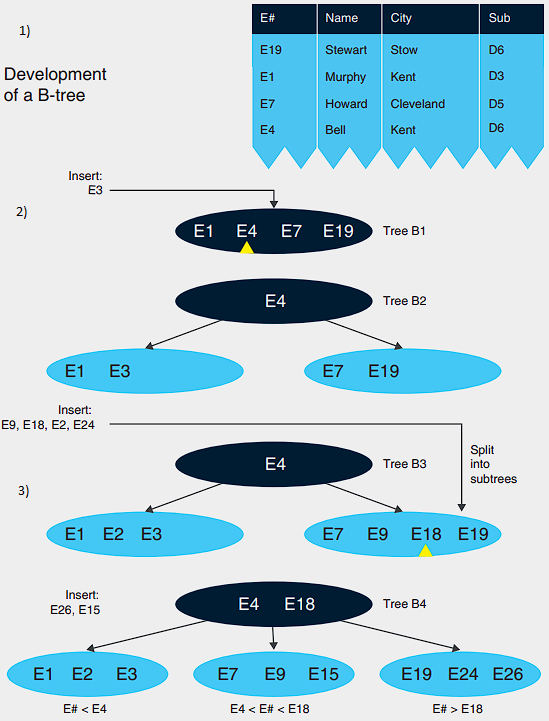
\includegraphics[width=0.7\textwidth]{images/btree.png}
    \caption{B-tree в динамике}
    \label{img2}
\end{figure}
\newpage
Время доступа используя B-tree напрямую зависит от его высоты. Как было показано высоту можно компенсировать увеличиваем количества поддеревьев.
\subsubsection{Методы хеширования}
\end{document}